\documentclass[12pt]{article}
\usepackage{enumitem}
\usepackage{amsmath}
\usepackage{amsfonts}
\usepackage{graphicx}
\usepackage{multirow}
\usepackage[margin=0.5in]{geometry}
\renewcommand{\thesubsection}{\alph{subsection}.}
\begin{document}
\title{CSCI 567 Fall 2016 \\Homework 2}
\author{MohammedJunaid Hundekar \\2548-4069-96 \\hundekar@usc.edu\\
	   Collaborators: Sagar Makhwana, Dhawal Shah, Ankit Kothari}
\maketitle
\section{Logistic Regression}
\begin{enumerate}[label=\alph*.]
    \item Negative Log Likelihood as loss function:
    Consider the  probability of a single training sample $(x_n,y_n)$\\
	\begin{align}
	 	p(y_n|x_n;b;w) &= \sigma(b+w^T x_n) \hspace{15mm}   if y_n = 1\\
        p(y_n|x_n;b;w) &= 1 - \sigma(b+w^T x_n) \hspace{9mm} if y_n = 0\\
        p(y_n|x_n;b;w) &= \sigma(b+w^T x_n)^{y_n}   [1 - \sigma(b+w^T x_n)]^{1-y_n}\\
        L(P(D)) &= \prod_n \{ \sigma(b+w^T x_n)^{y_n}   [1 - \sigma(b+w^T x_n)]^{1-y_n} \}
	\end{align}\\
    Taking log likelihood on the whole training set of size D$(x_1,y_1), (x_2,y_2),...(x_n,y_n)$\\
    \begin{align}
    \log L(P(D)) &= \sum_n \{ y_n\log \sigma(b+w^T x_n) + (1-y_n) \log[1 - \sigma(b+w^T x_n)] \}
    \end{align}
    Taking negative of the log likelihood\\
    \begin{align}
    \varepsilon(b,w) = - \sum_n \{ y_n\log \sigma(b+w^T x_n) + (1-y_n) \log[1 - \sigma(b+w^T x_n)] \}
	\end{align}
    For convenience\\ 
    Append 1 to $x \hspace{3mm} [1 \hspace{5mm} x_1 \hspace{5mm} x_2 \hspace{5mm} x_3 \hspace{5mm} ... \hspace{5mm} x_n]$\\
    Append b to $w \hspace{3mm} [b \hspace{4mm} w_1 \hspace{5mm} w_2 \hspace{5mm} w_3 \hspace{4mm} ... \hspace{4mm} w_n]$\\
Negative Log likelihood simplifies to\\
\begin{align}
\varepsilon(b,w) = - \sum_n \{ y_n\log \sigma(w^T x_n) + (1-y_n) \log[1 - \sigma(w^T x_n)] \}
\end{align}
\newpage
\item Gradient Descent Model
Consider $\sigma(a) = \frac{1}{1+e^{-a}}$\\ \\
$\frac{d\sigma(a)}{da} = \sigma(a)[1 - \sigma(a)]$\\\\
$\frac{d\log \sigma(a)}{da} = 1 - \sigma(a)$\\\\
Taking derivative of equation 7 w.r.t $w$\\
\begin{align}
\frac{\partial \varepsilon(w) }{\partial w} &= - \sum_n \{ y_n[1-\sigma(w^T x_n)]x_n (1-y_n) \sigma (w^T x_n)x_n\}\\
\frac{\partial \varepsilon(w) }{\partial w} &= \sum_n \{ \sigma(w^Tx_n) - y_n \}x_n\\
w^{(t+1)} &= w^{(t)} - \eta \sum_n \{ \sigma(w^T x_n) -y_n \} x_n \hspace{10mm} \eta > 0
\end{align}
Gradient descent works by updating the weights by using equation 10.\\
For the gradient descent to converge we need to select the step size ($\eta$) carefully.\\
If $\eta$ is too small then the algorithm will take a long time to converge, on the other hand if $\eta$ is too long the algorithm will oscillate and may not converge.
\item Log Likelihood Multi-Class logistic regression
Given
\begin{align}
P(Y=k|X=x) &= \frac{\exp (w_k^T x)}{1+\sum_1^{k-1}\exp (w_t^T x)} \hspace{10mm} \textrm{ for k=1,2...k-1}\\
P(Y=k|X=x) &= \frac{1}{1+\sum_1^{k-1}\exp (w_t^T x)} \hspace{10mm} \textrm{ for k=K}
\end{align}
We can simplify the above expression by introducing another fixed parameter $w_k = 0$\\
Thus we get\\
\begin{align}
P(Y=k|X=x) &= \frac{\exp (w_k^T x)}{\sum_1^{K-1}\exp (w_t^T x)} \hspace{10mm} \textrm{ for k=1,2...k-1}\\
P(Y=k|X=x) &= \frac{1}{\sum_1^{K-1}\exp (w_t^T x)} \hspace{10mm} \textrm{ for k = K}\\
P(Y=k|X=x) &= \frac{\exp (w_k^T x)}{\sum_1^{K}\exp (w_t^T x) } \hspace{10mm} \textrm{By adding 13 and 14}
\end{align}
Let us $y_n$ by an vector $\boldsymbol y_{n} = [y_{n1} \hspace{5mm} y_{n2} \hspace{5mm} y_{n3} \hspace{5mm} y_{n4} \hspace{5mm} ... \hspace{5mm} y_{nK}]^T$\\
Where \\$y_{nk} = 1 \hspace{10mm} \textrm{if $y_n = k$}$\\
$y_{nk} = 0$ \hspace{8mm} otherwise\\
Taking the negative of the log likelihood
\begin{align}
- \log L(P(D)) &= -\sum_n  \log P(y_n|x_n)\\
&= -\sum_n \log \prod_{k=1}^K P(C_k|x_n)^{y_{nk}}\\
&= -\sum_n \sum_k y_{nk} \log P(C_k|x_n)\\
&= \sum_n \sum_k y_{nk} \log (\frac{\exp (w_k^T x)}{\sum_1^{K}\exp (w_t^T x) })\\
l(w_1,w_2...w_k)&= -\sum_{i=1}^n \sum_k y_{ik} \log P(y= y_{ik}|x = x_i)\\
l(w_1,w_2...w_k)&= - \sum_n \sum_k y_{nk}[ w_k^T x - \log (\sum_1^{K}\exp (w_t^T x)) ]
\end{align}
\item Gradient Descent of (c)
Taking derivative of 20 w.r.t $\partial w_i$\\
\begin{align}
\frac{\partial - l(w_1,w_2...w_k)} {\partial w_i} &=  \sum_n[\frac{\exp (w_i^T x)}{\sum_1^{K}\exp (w_t^T x)}x_i - x_i y_{ki}]\\
& = \sum_n (x_i[P(Y=y_{ki}|X=x_i) - y_{ki}])
\end{align}
Update rule for w
\begin{align}
w_k \leftarrow w_k - \sum_i(P(Y=y_{ki}|X=x_i) - y_{ki})x_i
\end{align}
\end{enumerate}
\section{Linear/Gaussian Discriminant}
\begin{enumerate}[label=\alph*.]
\item 
Given: $D = \{ (x_n,y_n)\}_{n=1}^N; \hspace{9mm} y_n \in \{1,2\} $
\begin{align}
p(x_n,y_n) &= p(y_n) p(x_n)\\
&= p_1 \frac{1}{\sqrt[]{2\pi}\sigma_1} \exp\bigg( - \frac{(x_n-\mu_1)^2}{2\sigma_1^2}\bigg) \hspace{5mm}if y_n =1\\
&= p_2 \frac{1}{\sqrt[]{2\pi}\sigma_2} \exp\bigg( - \frac{(x_n-\mu_2)^2}{2\sigma_2^2}\bigg) \hspace{5mm}if y_n =2\\
\log P(D) &= \sum_n \log p(x_n,y_n)\\
&= \sum_{n:y_n=1} \log \bigg( p_1 \frac{1}{\sqrt[]{2\pi}\sigma_1} \exp\bigg( - \frac{(x_n-\mu_1)^2}{2\sigma_1^2}\bigg) \bigg) +\sum_{n:y_n=2} \log \bigg( p_2 \frac{1}{\sqrt[]{2\pi}\sigma_2} \exp\bigg( - \frac{(x_n-\mu_2)^2}{2\sigma_2^2}\bigg) \bigg)\\
&= \sum_{n:y_n=1} (\log p_1 - \log \sqrt[]{2\pi}\sigma_1 - \frac{(x_n-\mu_1)^2}{2\sigma_1^2} ) + \sum_{n:y_n=2} (\log p_2 - \log \sqrt[]{2\pi}\sigma_1 - \frac{(x_n-\mu_2)^2}{2\sigma_2^2} )
\end{align}
Now we can maximize $\{p_1,\mu_1,\sigma_1, p_2,\mu_2,\sigma_2\}$ separately from the above equation by taking derivative and equating to zero for each term.\\

\begin{align}
p_2 &= 1 - p_1\\
\frac{d l(D)}{dp_1} &= \frac{\sum_{n:y=1}1}{p_1} - \frac{\sum_{n:y=2}1}{1 - p_1} = 0\\
\frac{N_{y=1}}{p_1} &= \frac{N_{y=2}}{1 - p_1}\\
p_1 &= \frac{N_{y=1}}{N}\\
\textrm{Similarly,}\hspace{5mm} p_2 &= \frac{N_{y=2}}{N}\\
\frac{d l(D)}{d\mu_1} &= \sum_{n:y=1}[\frac{-2(x_n-\mu_1)(-1)}{2\sigma_1^2}] = 0\\
\sum_{n:y=1}(1)\mu_1 &= \sum_{n:y=1}x_n \\
\mu_1 &= \frac{\sum_{n:y=1}x_n}{N_{y=1}}\\
\textrm{Similarly,}\hspace{5mm} \mu_2 &= \frac{\sum_{n:y=2}x_n}{N_{y=2}}\\
\frac{d l(D)}{d\sigma_1} &= \sum_{n:y=1}\bigg([\frac{-1}{\sqrt[]{2\pi}\sigma_1}\sqrt[]{2\pi} ] - [\frac{(x_n-\mu_2)^2}{2\sigma_1^3}(-2)]\bigg)=0\\
\frac{\sum_{n:y=1}(x_n-\mu_2)^2}{\sigma_1^3} &= (\frac{\sum_{n:y=1}1}{\sigma_1})\\
\sigma_1^2 &= \frac{\sum_{n:y=1}(x_n-\mu_1)^2}{N_{y=1}}\\
\textrm{Similarly,}\hspace{5mm}\sigma_2^2 &= \frac{\sum_{n:y=2}(x_n-\mu_2)^2}{N_{y=2}}
\end{align}
\newpage
\item
Given 
$P(x|y=c_1) = \mathcal{N}(\mu_1,\Sigma)$ and
$P(x|y=c_2) = \mathcal{N}(\mu_2,\Sigma)$\\
Assume $ P(y=1) = \pi; \hspace{10mm} P(y=2) = 1-\pi  $
\begin{align}
P(x|y=1) &= \frac{1}{(2\pi)^{n/2}|\Sigma|^{1/2}} \exp \bigg(-\frac{1}{2}(x-\mu_1)^T\Sigma^{-1}(x-\mu_1) \bigg)\\
P(x|y=2) &= \frac{1}{(2\pi)^{n/2}|\Sigma|^{1/2}} \exp \bigg(-\frac{1}{2}(x-\mu_2)^T\Sigma^{-1}(x-\mu_2) \bigg)\\
P(y=1|x) &= \frac{P(x|y=1) P(y=1)}{P(x|y=1) P(y=1)+ P(x|y=2) P(y=2)} \\
&=\frac{1}{1+\frac{P(x|y=2) P(y=2)}{P(x|y=1) P(y=1)}}\\
& = \frac{1}{1 + \exp (-\frac{1}{2}(x-\mu_2)^T\Sigma^{-1}(x-\mu_2)  + \frac{1}{2}(x-\mu_1)^T\Sigma^{-1}(x-\mu_1) ) \frac{1-\pi}{\pi}}\\
& =  \frac{1}{1 + \frac{1-\pi}{\pi} \exp(\sum_{i=1}^N [\frac{(x_i-\mu_{1i})^2}{2\sigma_i^2} - \frac{(x_i-\mu_{2i})^2}{2\sigma_i^2}] } \\
&= \frac{1}{1+ \exp \bigg[\ln\frac{1-\pi}{\pi}+ \sum_i\bigg(x_i \frac{\mu_{2i} - \mu_{1i}}{\sigma_i^2} + \frac{\mu_{1i}^2 - \mu_{2i}^2}{2\sigma_i^2}\bigg) \bigg]}\\
\theta_1 &= - (\ln (\frac{1-\pi}{\pi}) + \sum_i\big(\frac{\mu_{2i}^2 - \mu_{1i}^2}{2\sigma_i^2}\big))\\
\theta_2 &= - (\sum_i\big(\frac{\mu_{1i} - \mu_{2i}}{\sigma_i^2}\big))\\
P(Y=1|x) &= \frac{1}{1+\exp(-\theta_1 - \theta_2 X)} \\
P(Y=1|x) &= \frac{1}{1+\exp(-\theta^T X)}
\end{align}
Appending a 1 in  $X \leftarrow [1 \hspace{5mm}x_1\hspace{5mm}x_2\hspace{5mm}...\hspace{5mm}x_n ]$ and $\theta = \theta_1 + \theta_2$
\end{enumerate}
\newpage
\section{Programming - Linear Regression}
\subsection*{3.1 Data Analysis}
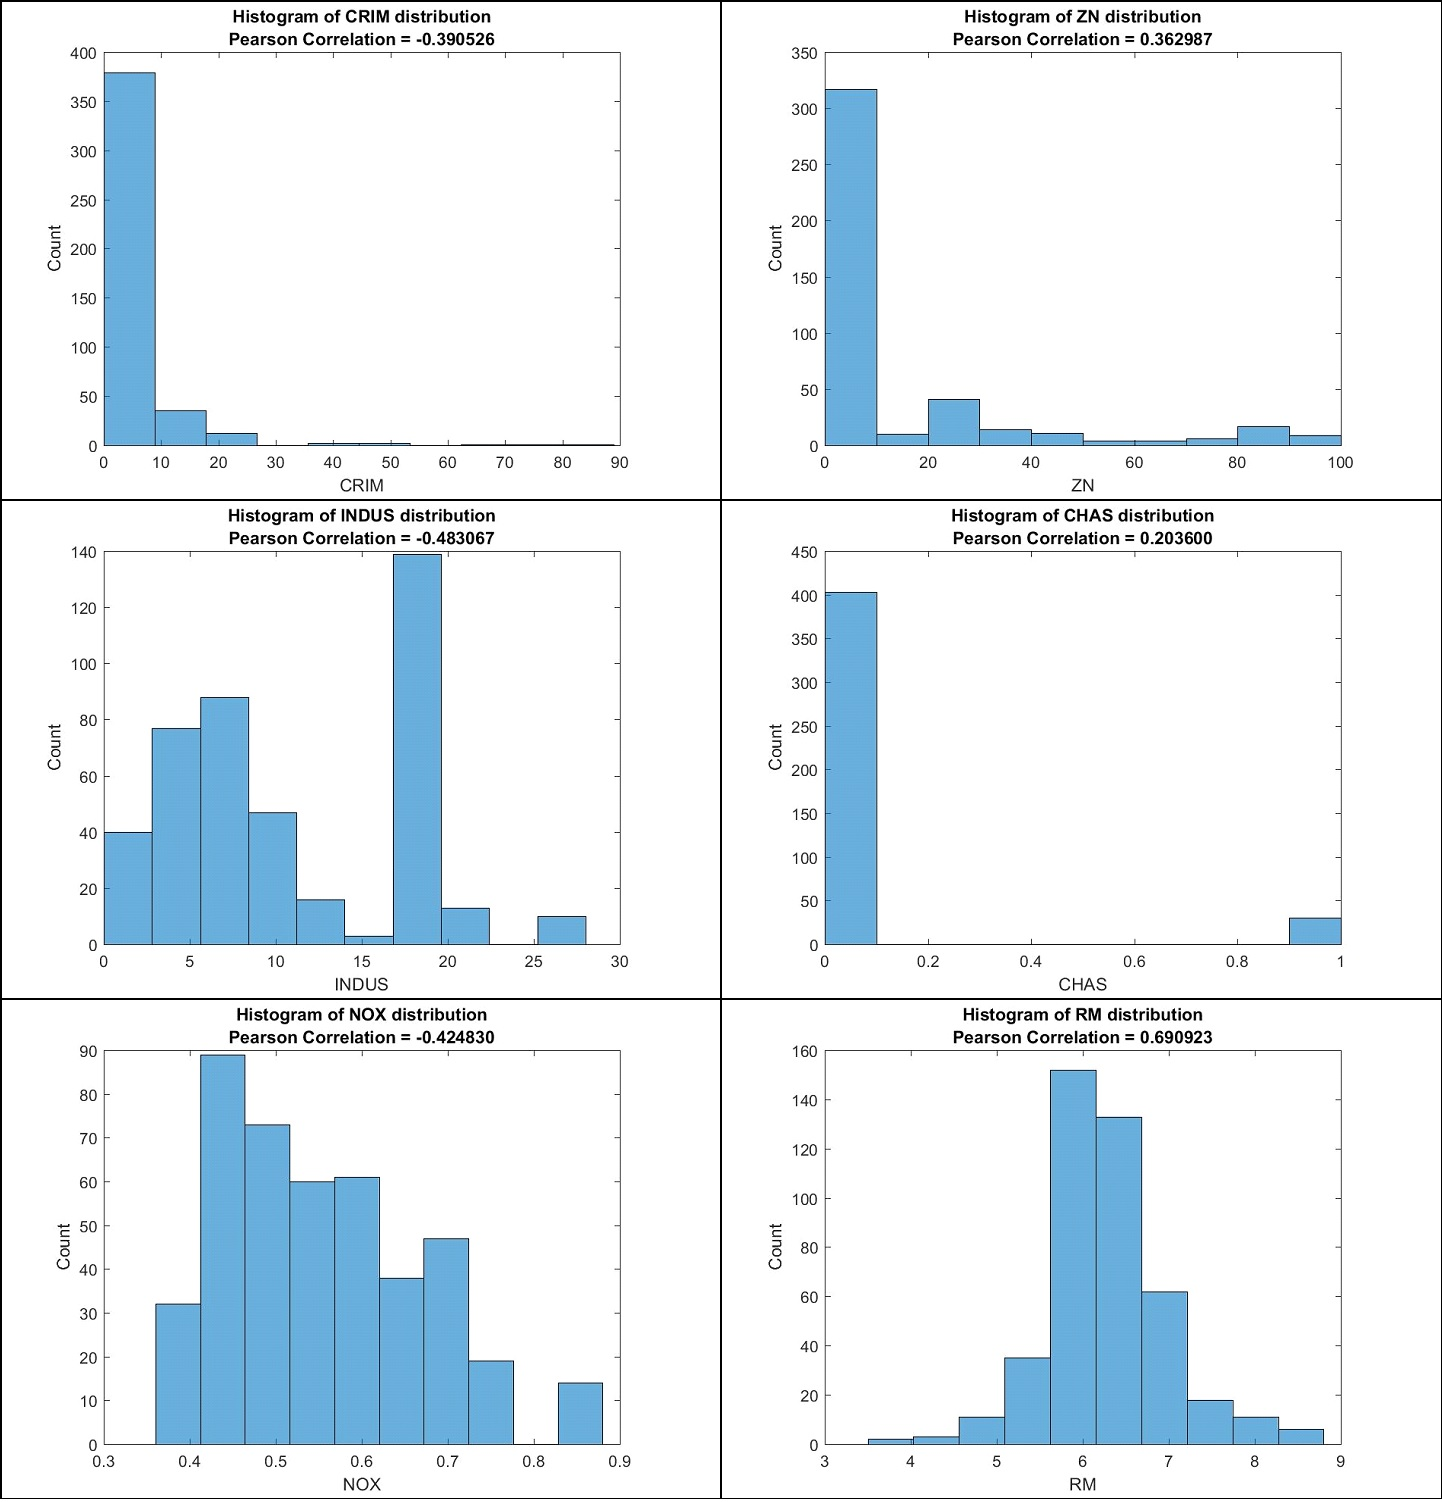
\includegraphics[width=\textwidth]{Hist1.jpg}
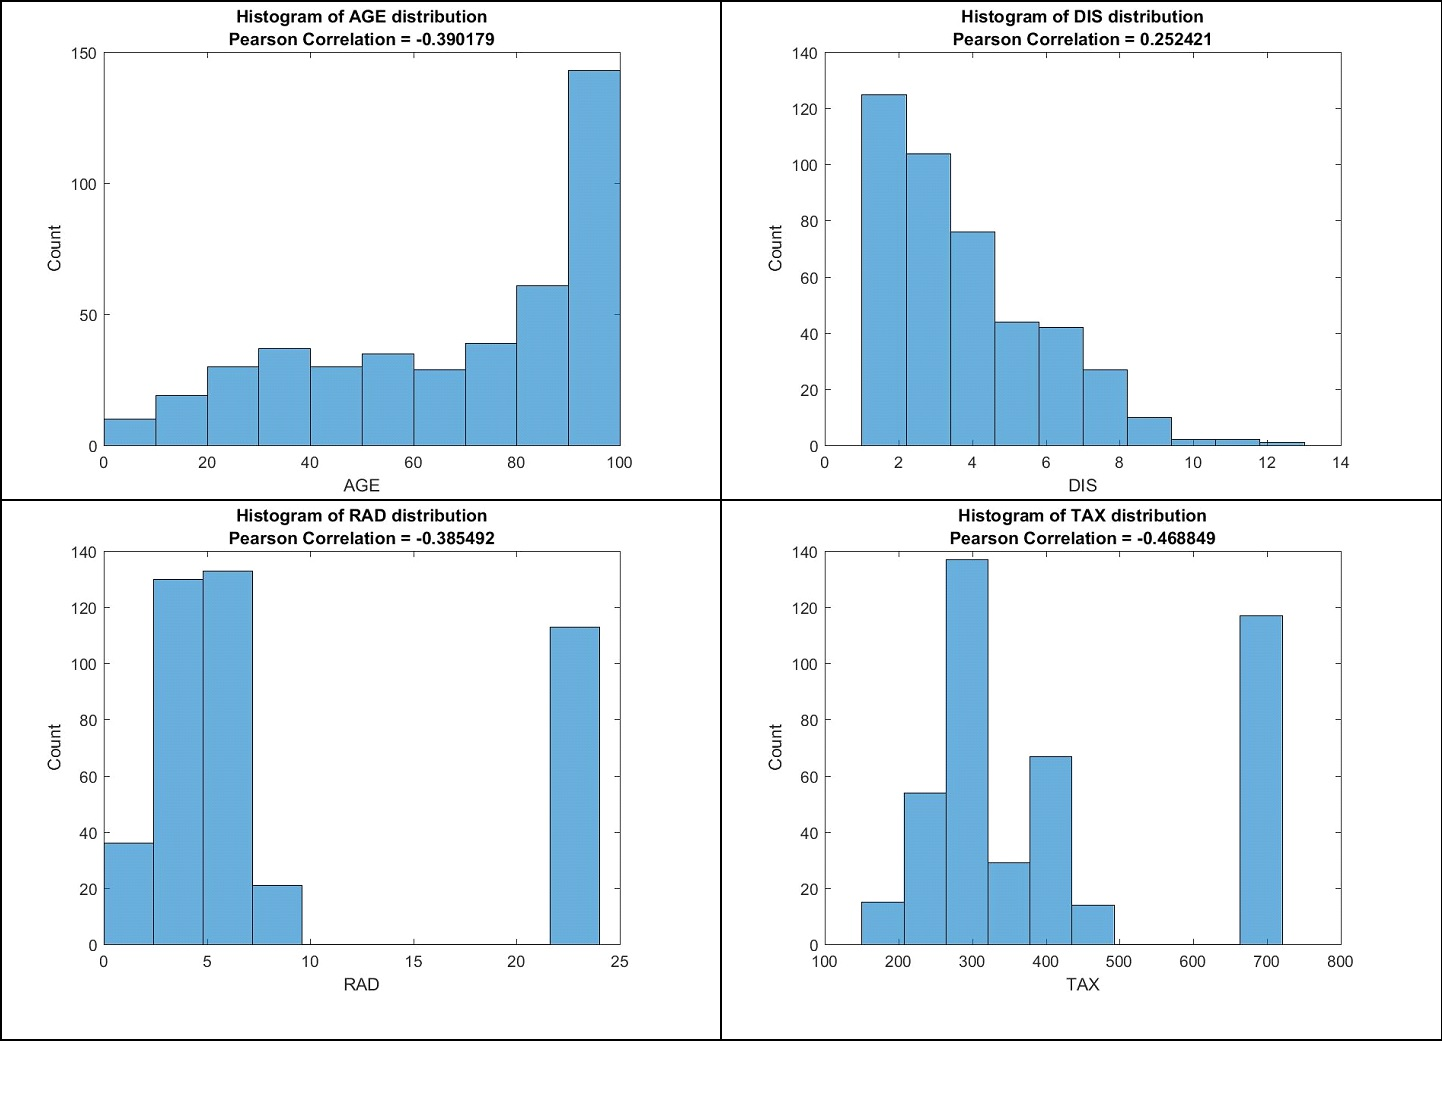
\includegraphics[width=\textwidth]{Hist2.jpg}
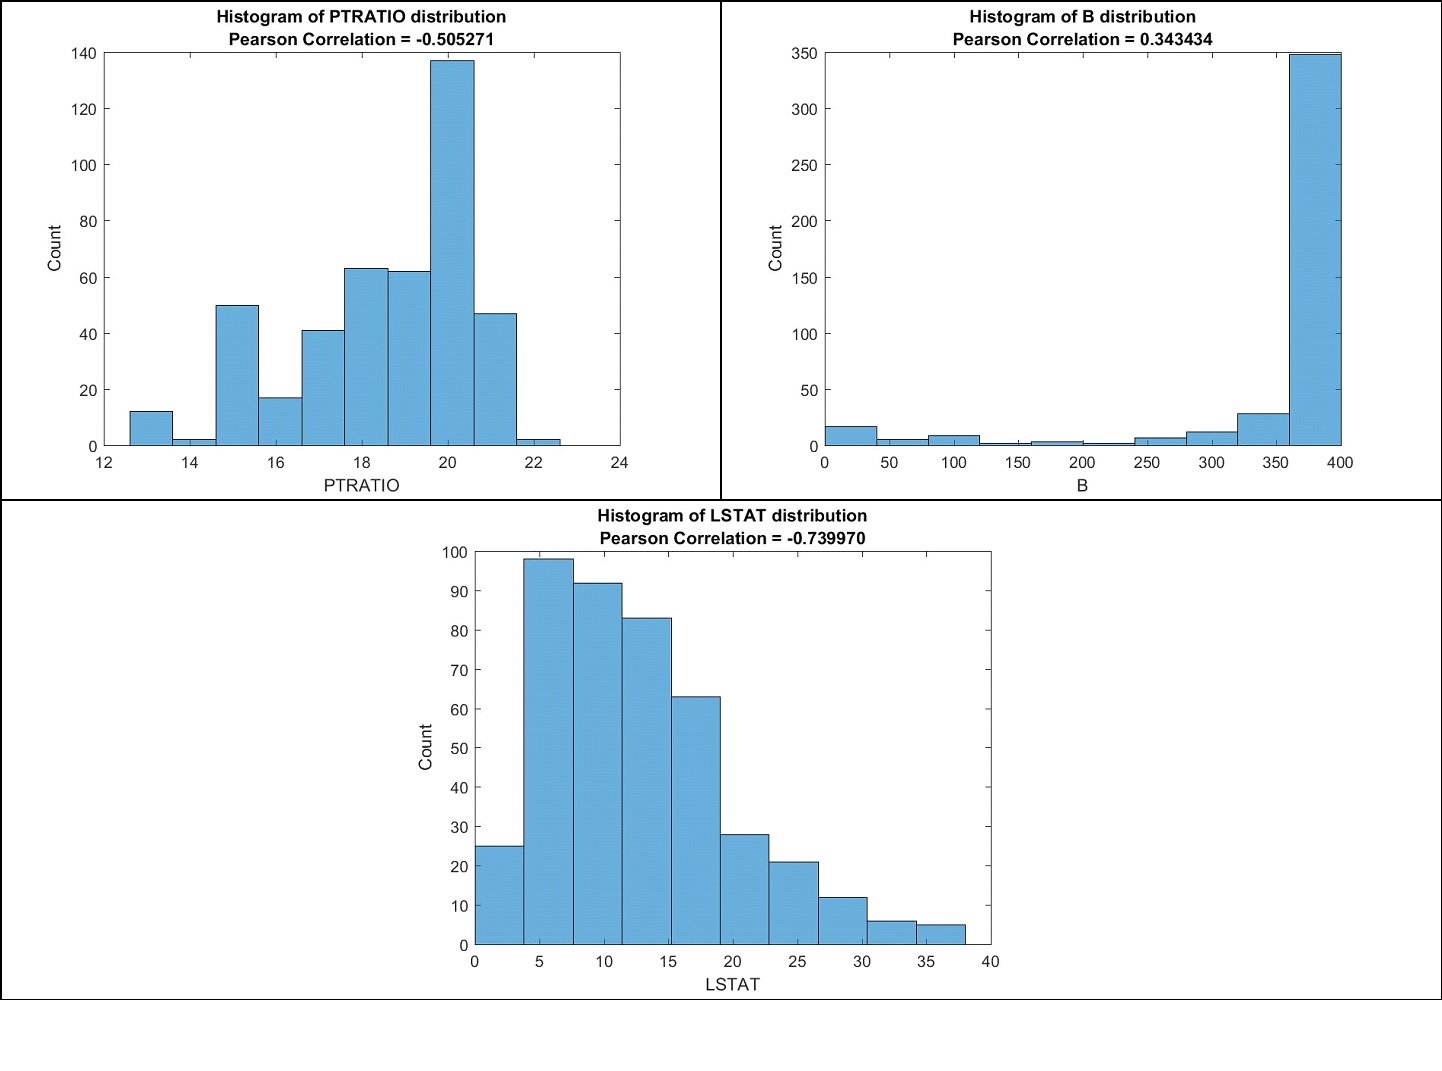
\includegraphics[width=\textwidth]{Hist3.jpg}
\subsection*{3.2 Linear Regression}
\begin{table}[h]
\centering
\caption{Linear and Ridge Regression Performance on Training and Test Data}
\label{Linear and Ridge Regression}
\begin{tabular}{|l|l|l|}
\hline
\textbf{Algorithm}        & \textbf{Training Set MSE} & \textbf{Testing Set MSE} \\ \hline
Linear Regression         & 20.9441                   & 28.4368                  \\ \hline
Rigde Regression  L =0.01 & 20.9441                   & 28.4371                  \\ \hline
Rigde Regression  L =0.10 & 20.9442                   & 28.4405                  \\ \hline
Rigde Regression  L =1.00 & 20.948                    & 28.476                   \\ \hline
\end{tabular}
\end{table}
\newpage
\textbf{Ridge Regression with Cross-Validation:}\\
Incrementing $ \lambda $ by 0.01 after each iteration. Displaying only every $ 100^{th} $ row for conciseness. See variable \textbf{Res\_cv}  for all values.
\begin{table}[h]
\centering
\caption{Lamda and MSE on Training Data }
\label{lamda vs mse}
\begin{tabular}{|l|l|}
\hline
\textbf{Lamda Value} & \textbf{MSE} \\ \hline
0.0001               & 32.887567    \\ \hline
0.9801               & 32.790939    \\ \hline
1.9801               & 32.716183    \\ \hline
2.9801               & 32.66416     \\ \hline
3.9801               & 32.633673    \\ \hline
4.9801               & 32.623659    \\ \hline
5.9801               & 32.633161    \\ \hline
6.9801               & 32.661308    \\ \hline
7.9801               & 32.707307    \\ \hline
8.9801               & 32.770422    \\ \hline
9.9801               & 32.849976    \\ \hline
\end{tabular}
\end{table}
\begin{figure}[h]
\includegraphics[width=\textwidth, width=15cm, height=10cm]{Lamda_VS_MSE.jpg}
\centering
\end{figure}
\newpage
\begin{table}[t]
\centering
\caption{ Results of Cross validation on Testing Set}
\label{CV Result}
\begin{tabular}{|l|l|}
\hline
\textbf{Lamda Value} & \textbf{MSE} \\ \hline
4.990100               & 28.671087    \\ \hline
\end{tabular}
\end{table}
From the graph we can see that when $ \lambda = 4.990100 $ we get the minimum MSE on Training Data:\\ MSE = 32.623659.\\
Choosing this, we get MSE = 28.671087 on the testing set.
\subsection*{3.3 Feature Selection}
\subsection{ Four features with highest absolute correlation}
\begin{table}[h]
\centering
\caption{Features with highest absolute correlation}
\label{4_correlation}
\begin{tabular}{|l|l|l|}
\hline
\textbf{Attribute} & \textbf{Name} & \textbf{Correlation} \\ \hline
13                 & LSTAT         & 0.74                 \\ \hline
6                  & RM            & 0.6909               \\ \hline
11                 & PTRATIO       & 0.5053               \\ \hline
3                  & INDUS         & 0.4831               \\ \hline
\end{tabular}
\end{table}
Using the above 4 features to train the linear regression\\
MSE on training data:: 26.406604\\
MSE on Testing data:: 31.496203\\
\subsection{ Four features with highest absolute correlation with Residue}
\begin{table}[h]
\centering
\caption{Features and their correlation with Residue }
\label{corr_residue}
\begin{tabular}{|l|l|l|}
\hline
\textbf{Attribute} & \textbf{Name} & \textbf{Correlation} \\ \hline
13                 & LSTAT         & 0.74                 \\ \hline
6                  & RM            & 0.3709               \\ \hline
11                 & PTRATIO       & 0.2975               \\ \hline
4                  & CHAS          & 0.2196               \\ \hline
\end{tabular}
\end{table}
Using the above 4 features to train the linear regression\\
MSE on training data:: 25.106022\\
MSE on Testing data:: 34.600072\\
\subsection*{Selection with Brute-force Search}
The columns that give MIN MSE: 25.106022 on Training SET: [4     6    11    13]\\
Corresponding MSE: 34.600072 on Testing SET\\
\\The columns that give MIN MSE: 30.100406 on Testing SET: [6    11    12    13]\\
Corresponding value of MSE: 25.744417 on Training SET\\
\subsection*{3.4 Polynomial Feature Expansion}
Expanding the existing features by polynomial expansion $x_i * x_j \{i,j=1, 2, 3 ... 13\}$ to get 104 features.
The result of training the linear regression model on these feature are:\\
MSE on Training data:: 5.077346\\
MSE on Testing data:: 14.559306\\
\end{document}